\documentclass[../TDTM3.tex]{subfiles}%

\begin{document}
\section[s]"3"{Utilisation de la méthode différentielle}
\label{sec:mtdiff}
\enonce{%
	La réaction étudiée est l'oxydation des ions iodure par les ions ferriques
	Fe(III). Les couples d'oxydoréduction mis en jeu sont les couples
	$\ce{I2}/\ce{I-}$ et $\ce{Fe^{3+}}/\ce{Fe^{2+}}$, toutes les espèces étant
	dissoutes dans l'eau.
}

\QR{%
	Écrire l'équation-bilan de l'oxydation des ions iodure par les ions
	fer (III), en affectant les espèces du fer du nombre stœchiométrique 1.
	Si la concentration d'ions iodure passe de $c_0$ à $c_0 - x$ entre 0 et
	$t$, comment définit-on par rapport à $x$ la vitesse volumique de la
	réaction~?
}{%
	\begin{tcn}(data)<lfnt>{Données}
		Même sans connaître le principe de l'oxydo-réduction, la réaction
		étudiée met en contact les ions iodure, donc $\ce{I-}$, et les ions
		fer III, donc $\ce{Fe^{3+}}$. Par déduction les produits sont les
		autres composés cités, c'est-à-dire $\ce{I2}$ et $\ce{Fe^{2+}}$. La
		manière la plus simple de l'équilibrer serait avec des nombres
		entiers et notamment $2$ devant chaque élément sauf $\ce{I2}$, mais
		on nous demande de l'écrire avec un nombre stœchiométrique de $1$
		devant les espèces du fer.
	\end{tcn}
	En tant qu'équation-bilan et donc qu'équation, il suffit de diviser
	chaque côté par 2 pour obtenir~:
	\begin{tcn}(rslt)<lfnt>{Résultat}
		\[\ce{Fe^{3+}_{\aqu} + I^{-}_{\aqu} = Fe^{2+}_{\aqu} +
			1/2I2_{\aqu}}\]
	\end{tcn}
	Il n'est en effet pas choquant d'avoir des coefficients stœchiométriques
	qui ne sont pas entiers dans une équation-bilan.
	\bigbreak
	\begin{tcn}(rapp)<lfnt>{Outil}
		Or, par le lien vitesse-concentration, on a
		\[v = \frac{1}{\nu_i} \dv{[\ce{X}_i]}{t}\]
		pour X$_i$ un élément de l'équation-bilan
		\[0 = \sum_{i} \nu_i\ce{X}_i\]
	\end{tcn}
	\begin{tcn}(appl)<lfnt>{Application}
		Si on veut exprimer $v$ en fonction de la concentration en ions iodure,
		on a donc
		\begin{gather*}
			v = \frac{1}{-1} \dv{[\ce{I-}]}{t}
			= - \dv{c_0 - x}{}
			\Leftrightarrow
			\boxed{v = \dv{x}{t}}
		\end{gather*}
		étant donné que $c_0$ est une constante.
	\end{tcn}
}

\QR{%
	On suppose une cinétique avec ordre, de constante de vitesse $k$~; on note $p$
	l'ordre partiel par rapport aux ions fer (III) et $q$ l'ordre partiel par
	rapport aux ions iodure. Comment s'écrit la vitesse $v$~? Quelle est alors
	l'unité usuelle de $k$ (au besoin en fonction de $p$ et de $q$)~?
}{%
	Par définition,
	\begin{tcn}(tool)<lfnt>{Outil}
		Une réaction $a\ce{A} + b\ce{B} = c\ce{C} + d\ce{D}$ a une loi
		de vitesse admettant un ordre si elle s'écrit
		\[v = k[\ce{A}]^{p}[\ce{B}]^{q}\]
		avec $p$ l'ordre partiel par rapport au réactif A et $q$ l'ordre partiel par
		rapport au réactif B.
	\end{tcn}
	\begin{tcn}(prop)<lfnt>{Résultat}
		Ici, les réactifs sont les ions fer III et les ions iodure, donc la vitesse
		s'écrirait donc
		\[
			\boxed{
			v = k [\ce{Fe^{3+}}]^p[\ce{I^{-}}]^q
			}
		\]
	\end{tcn}
	\begin{tcn}(appl)<lfnt>{Application}
		On trouve l'unité de $k$ en étudiant celles des termes en jeu dans
		l'équation~:
		\[\si{mol.L^{-1}.s^{-1}} = [k]\times (\si{mol.L^{-1}})^{a+b}\]
		donc la dimension de $k$ est
		\fbox{$(\si{mol.L^{-1}})^{1-a-b}\si{s^{-1}}$}.
	\end{tcn}
}
\QR{%
	À la date $t$ après le mélange d'une solution d'iodure de potassium
	avec une solution ferrique, on prélève à la pipette \SI{5}{mL} de
	solution et on dilue 10 fois avant de procéder à un dosage de la quantité
	d'iode formée. Justifier l'intérêt cinétique de cette dilution.
}{%
	Dans la dernière partie du cours, nous avons introduit le concept du dosage
	par titrage, et exposé la nécessité de \textbf{ralentir la
		réaction} pour qu'un volume de solution prélevé à un instant $t$ mais
	dosé par méthode chimique à un instant ultérieur ait une évolution négligeable
	entre ces deux instants~: cette pratique s'appelle la
	\textbf{trempe chimique}, et une des manières de réaliser une trempe
	chimique est de fortement diluer la solution prélevée. En effet, la vitesse
	étant reliée à la concentration en les réactifs (pour une réaction admettant
	un ordre), on peut «~geler~» l'état de la réaction en augmentant le volume du
	solvant et donc en réduisant la concentration des éléments.
}

\QR{%
	Les résultats d'une série de mesures sont présentés ci-dessous, $x$ se
	rapportant à la quantité d'ions iodure qui ont été oxydés dans le milieu
	réactionnel à la date du prélèvement.
	\begin{center}
		\begin{tabular}{lccccc}
			\toprule
			$t(\si{s})$                 &
			60                          & 120 & 180 & 240 & 300 \\
			\midrule
			$x(\si{\micro mol.L^{-1}})$ &
			13                          & 25  & 36  & 46  & 55  \\
			\bottomrule
		\end{tabular}
	\end{center}
	Que représente la grandeur $x(t)/t$~? Pourquoi diminue-t-elle en cours
	de réaction~? Représenter graphiquement cette grandeur en fonction de
	$t$ à partir du tableau ci-dessus, avec en abscisse $t \in
		\SIrange{0}{300}{s}$~; en déduire une estimation de la valeur initiale
	$\left.\dv{x}{t}\right|_0$.
}{%
	\begin{minipage}{0.45\linewidth}
		\begin{center}
			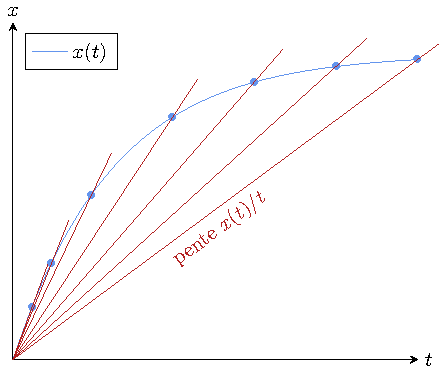
\includegraphics[width=\linewidth]{xtt}
		\end{center}
	\end{minipage}
	\hfill
	\begin{minipage}{0.45\linewidth}
		On peut commencer par remarquer que $x(t)/t$ a la dimension d'une
		vitesse de réaction, en $\si{mol.L^{-1}.s^{-1}}$. Il faut ensuite
		remarquer que $x(t)/t = (x(t) - x(0))/(t-0)$ avec un avancement nul
		à $t=0$~; si $t$ est suffisamment petit, on a donc
		\[ \frac{x(t)}{t} \approx \left.\dv{x}{t}\right|_0\]
		et ainsi $x(t)/t$ est une approximation de la vitesse de la
		réaction~; c'est ce qu'on appelle l'approximation de la tangente par
		la sécante. En faisant la régression linéaire jusqu'en 0, on
		trouvera bien la vitesse en 0.
	\end{minipage}

	On réalise cette régression avec $y = x(t)/t$, $x = t$ et $b = v_0$,
	pour obtenir le résultat suivant~:
	\begin{minipage}{0.45\linewidth}
		On trouve alors, grâce à l'ordonnée à l'origine,
		\[\boxed{v_0 = \SI{2.25e-7}{mol.L^{-1}.s^{-1}}}\]
	\end{minipage}
	\begin{minipage}{0.55\linewidth}
		\begin{center}
			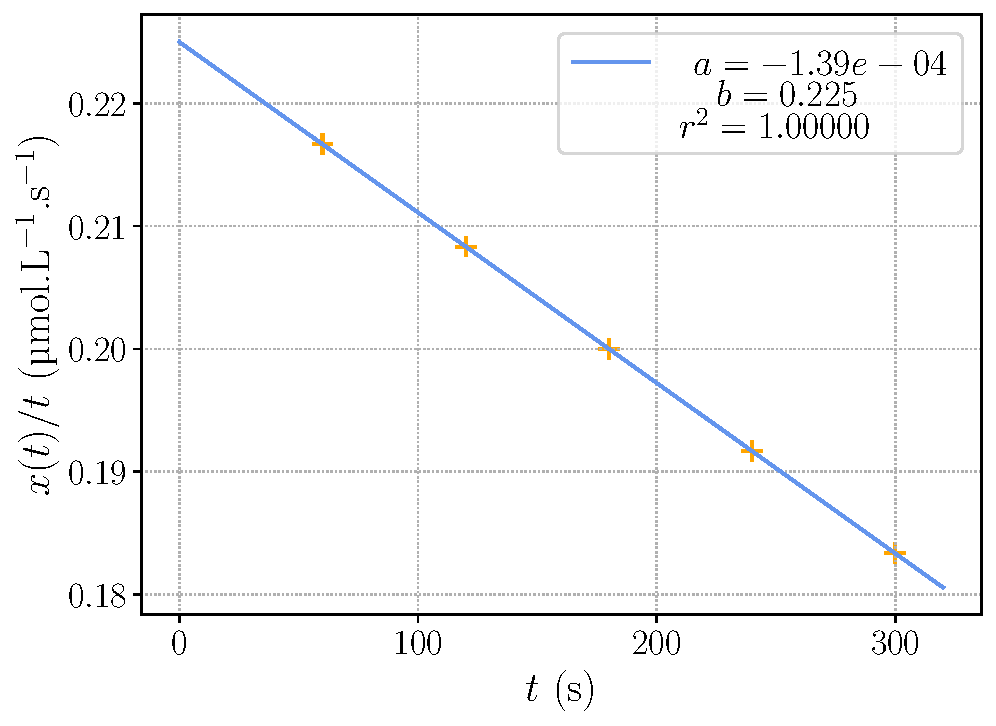
\includegraphics[width=\linewidth]{exo3_xtt}
		\end{center}
	\end{minipage}
}

\QR{%
	Grâce à la méthode précédente, on détermine les valeurs initiales de
	$\dv{x}{t}$ pour différentes concentrations initiales des deux réactifs.
	Quelques résultats sont présentés ci-dessous~:
	\begin{center}
		\begin{tabular}{lccccccc}
			\toprule
			$c_0 = [\ce{I-}]_0$               &
			$(\si{\micro mol.L^{-1}})$        &
			2                                 & 2          & 2          & 6  & 6  & 8   \\
			\midrule
			$[\ce{Fe^{3+}}]_0$                &
			$(\si{\micro mol.L^{-1}})$        &
			2                                 & 4          & 8          & 2  & 4  & 8   \\
			\midrule
			$\DS \eval{\dv{x}{t}}_{0}$        &
			$(\si{\micro mol.L^{-1}.s^{-1}})$ &
			\num{5.7}                         & \num{11.1} & \num{22.5} & 52 & 99 & 354 \\
			\bottomrule
		\end{tabular}
	\end{center}
	En déduire les valeurs de $p$ et $q$, supposées entières.
}{%
	Pour déterminer les valeurs de $p$ et $q$, il faut utiliser des
	expériences dans lesquelles l'une des deux concentrations est fixe alors
	que l'autre non~: ça revient au même principe que la dégénérescence de
	l'ordre.
	\bigbreak
	Ici, dans les expériences 1, 2 et 3 par exemple, on a $[\ce{I-}]_0 =
		\cte$. Dans ce cas, à chaque fois on a
	\begin{gather*}
		v_{0,1} = k[\ce{Fe^{3+}}]_{0,1}{}^p [\ce{I-}]_0{}^q\\
		v_{0,2} = k[\ce{Fe^{3+}}]_{0,2}{}^p [\ce{I-}]_0{}^q\\
		v_{0,3} = k[\ce{Fe^{3+}}]_{0,3}{}^p [\ce{I-}]_0{}^q
	\end{gather*}
	et $v_0$ ne dépend que de la concentration en ions fer III. Comme on
	cherche des ordres partiels entier, on en déduit qu'il suffit d'étudier
	comment varie $v_0$ à une modification simple de la concentration
	initiale en ions fer III pour déduire l'ordre~: ici par exemple, en
	multipliant par $2$ cette concentration initiale, la vitesse est
	multipliée par environ 2 à chaque fois. Le seul ordre partiel $p$
	permettant cette relation est bien évidemment un ordre partiel égal à
	1~: on en déduit \fbox{$p = 1$}.
	\bigbreak
	De même, avec des expériences où la concentration initiale en ions fer
	III est fixe, par exemple pour les 1 et 4, on a une variation de $v_0$
	dépendante uniquement de la concentration initiale en ions iodure. Or,
	on remarque cette fois que multiplier par 3 cette concentration multiplie
	par 9 la vitesse initiale~: le seul ordre partiel entier qui permet que
	$3^q = 9$ est bien évidemment 2, et on en déduit \fbox{$q = 2$}.
}
\QR{%
Déterminer la constante de vitesse $k$ définie à la question 2)~; on
précisera la méthode suivie pour utiliser au mieux les données.
}{%
On pourrait mesurer $k$ en prenant $v_0/([\ce{Fe^{3+}}]_{0}{}\times
	[\ce{I-}]_0{}^2)$ à chaque fois et en faisant la moyenne, mais pour
avoir la meilleure estimation avec ces données la régression linéaire
est plus efficace~: les éventuelles variabilités de mesure se combinent
toutes ensemble pour avoir une estimation combinée dépendante, plutôt
qu'une estimation moyennée où les valeurs sont supposées indépendantes.
Ainsi, on trace
\begin{gather*}
	v_0 = f([\ce{Fe^{3+}}]_{0}{}\times [\ce{I-}]_0{}^2)
\end{gather*}
dont le coefficient directeur sera $k$.

\begin{minipage}{0.45\linewidth}
	On trouve alors
	\begin{gather*}
		k = \SI{6.90e-1}{\micro mol^{-2}.L^2.s^{-1}}\\
		\Leftrightarrow \boxed{
		k = \SI{6.90e11}{mol^{-2}.L^2.s^{-1}}}
	\end{gather*}
\end{minipage}
\hfill
\begin{minipage}{0.55\linewidth}
	\begin{center}
		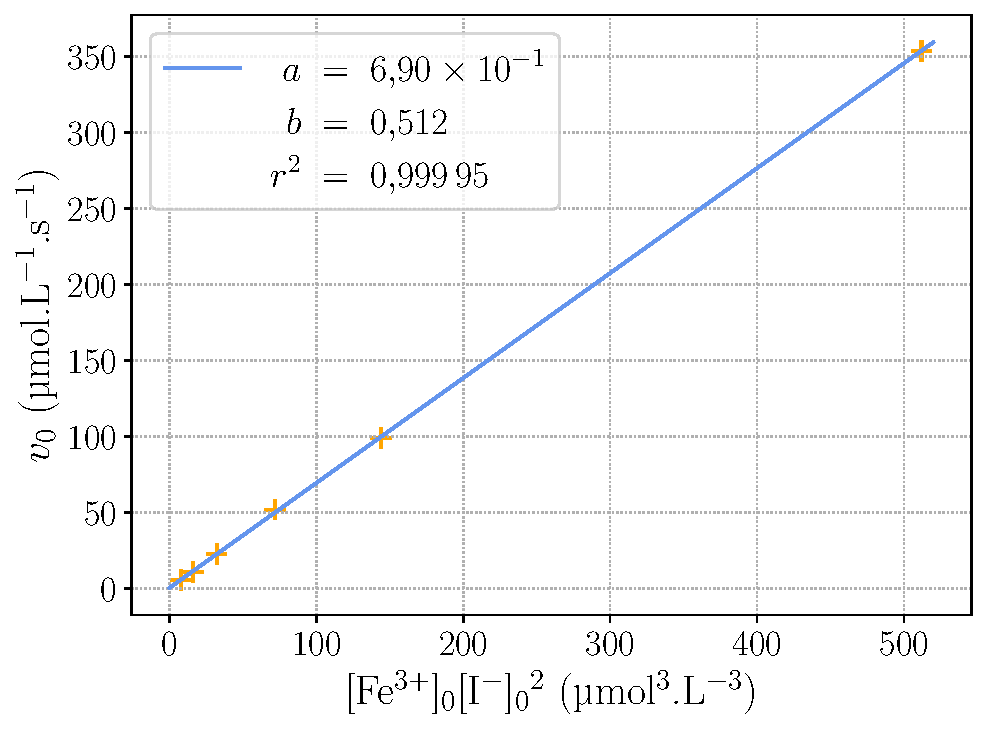
\includegraphics[width=\linewidth]{exo3_v0}
	\end{center}
\end{minipage}
}
\QR{%
	Dans l'hypothèse d'un état initial ne contenant que les deux réactifs à la
	même concentration $c_0$, établier la relation littérale donnant $x(t)$ sous
	la forme~:
	\begin{center}
		«~expression en $(x,c_0)$ = expression en $(k,t)$~»
	\end{center}
	En déduire la dépendance entre le temps de demi-réaction $\tau$ et la
	concentration $c_0$.
}{%
	\begin{tcn}(data)<lfnt>{Données}
		Les conditions de cette question sont celles des proportions
		stœchiométriques~: en effet, comme les deux réactifs ont le même coefficient
		stœchiométrique \textbf{et que celui-ci est égal à
			1}, leurs deux concentrations à un instant $t$ valent $c_0 -x$. Ainsi,
		la vitesse de réaction s'écrit
		\begin{gather*}
			v = k (c_0 - x)(c_0-x)^2 = k(c_0-x)^3 = \dv{x}{t}
		\end{gather*}
	\end{tcn}
	\begin{tcn}(appl)<lfnt>{Calcul}
		en la reliant à la question 1). Comme pour l'ordre 2, on résout cette
		équation en séparant les variables~:
		\begin{gather}\label{eq:difftrois}
			\frac{\dd x}{(c_0 -x)^3} = k\dt
		\end{gather}
	\end{tcn}
	\begin{tcn}(tool)<lfnt>{Outil}
		On doit, de cette équation, en trouver une primitive. Pour effectuer ce
		raisonnement, il est plus simple de partir d'une forme simple à dériver qui
		donnerait celle à gauche du signe égal. Or, on sait que pour $u$ une
		fonction,
		\[(u^{\alpha})' = \alpha u' u^{\alpha-1}\]
		Donc si $\alpha = -2$, on aura $u^{-3}$ en dérivant, ce qui correspond à
		notre équation à nous. Cependant, il faut faire attention aux constantes et
		signes $\pm$ dans de telles situations~: calculons la dérivée en entier.
		\[(u^{-2})' = -2 u' u^{-3}\]
		Soit
		\begin{gather*}
			\left.\begin{array}{rcl}
				u~: \Rb^+ & \rightarrow & \Rb^+   \\
				x         & \mapsto     & c_0 - x \\
			\end{array}\right.
			\Rightarrow
			\left.\begin{array}{rcl}
				\dd u : \Rb^+ & \rightarrow & \Rb^+  \\
				x             & \mapsto     & -\dd x \\
			\end{array}\right.
		\end{gather*}
		On a donc
		\[\dd((c_0 -x)^{-2}) = -2 (-\dd x) (c_0 - x)^{-3}\]
		Et en prenant la primitive de chaque côté,
		\[\int\dd((c_0 -x)^{-2}) = \int -2 (-\dd x) (c_0 - x)^{-3}\]
	\end{tcn}
	\begin{tcn}(rslt)<lfnt>{Résultat}
		On peut donc résoudre l'équation différentielle \ref{eq:difftrois} par
		intégration, pour obtenir
		\begin{gather*}
			\frac{1}{(c_0 - x)^2} = 2kt + K
			\qet
			\frac{1}{c_0{}^2} = K
			\qdonc \boxed{
			\frac{1}{(c_0-x)^2} - \frac{1}{c_0{}^2} = 2kt}
		\end{gather*}
	\end{tcn}
	\begin{tcn}(defi)<lfnt>{Définition}
		Or, par définition, le temps de demi-réaction est le temps au bout duquel
		l'avancement est à la moitié de sa valeur finale, c'est-à-dire $x(\tau) =
			x_f/2$.
	\end{tcn}
	\begin{tcn}(appl)<lfnt>{Calcul}
		Ici, on trouve donc
		\begin{gather*}
			x(\tau) = \frac{c_0}{2}
			\Leftrightarrow
			\frac{1}{(c_0 - \frac{c_0}{2})^2} - \frac{1}{c_0{}^2} = 2k\tau
			\Leftrightarrow
			\frac{4}{c_0{}^2} - \frac{1}{c_0{}^2} = 2k\tau\\
		\end{gather*}
	\end{tcn}
	\begin{tcn}(rslt)<lfnt>{Résultat}
		Soit finalement
		\[\boxed{\tau = \frac{3}{2kc_0{}^2}}\]
	\end{tcn}
}

\end{document}
